\documentclass[10pt]{article}

\usepackage[margin=0.75in]{geometry}
\usepackage{amsmath,amsthm,amssymb}
\usepackage{xcolor}
\usepackage{cancel}
\usepackage{graphicx}
\usepackage{changepage}
\usepackage{circuitikz}
\usepackage{pgfplots}
\usepackage{physics}
\usepackage{hyperref}
\usepackage{siunitx}
\usepackage[breakable]{tcolorbox}
\usepackage[inline]{enumitem}

\theoremstyle{definition}
\newtheorem{problem}{Problem}
\newtheorem{soln}{Solution}

\pgfplotsset{compat=newest}
\usetikzlibrary{lindenmayersystems}
\usetikzlibrary{arrows}
\usetikzlibrary{calc}

\definecolor{incolor}{HTML}{303F9F}
\definecolor{outcolor}{HTML}{D84315}
\definecolor{cellborder}{HTML}{CFCFCF}
\definecolor{cellbackground}{HTML}{F7F7F7}
\newcommand{\eq}{=}
\usetikzlibrary{positioning, fit, calc}
\pgfdeclarelayer{background}  
\pgfsetlayers{background,main}

\makeatletter
\newcommand{\boxspacing}{\kern\kvtcb@left@rule\kern\kvtcb@boxsep}
\makeatother
\newcommand{\prompt}[4]{
    \ttfamily\llap{{\color{#2}[#3]:\hspace{3pt}#4}}\vspace{-\baselineskip}
}

\newcommand{\thevenin}[2]{
  \begin{center}
    \begin{circuitikz} \draw
      (0,0) -- (2,0) to[battery1, l_=$V_{Th}\eq#1$] (2,2) 
      to[resistor, l_=$R_{Th}\eq#2$] (0,2)
      ;
      \draw [o-] (-.07,2.079);
      \draw [o-] (-.07,0.079);
    \end{circuitikz}
  \end{center}
}

\newcommand{\norton}[2]{
  \begin{center}
    \begin{circuitikz} \draw
      (0,0) -- (3,0) to[american current source, l_=$I_{N}\eq#1$] (3,2) -- (0,2) (2,0)
      to[resistor, l=$R_{N}\eq#2$] (2,2)
      ;
      \draw [o-] (-.07,2.079);
      \draw [o-] (-.07,0.079);
    \end{circuitikz}
  \end{center}
}

\newcommand{\highlight}[1]{\colorbox{yellow}{$\displaystyle #1$}}

\newcommand{\ti}[1]{\widetilde{#1}}

\hypersetup{
    colorlinks=true,
    linkcolor=blue,
    filecolor=magenta,      
    urlcolor=cyan,
    pdftitle={Overleaf Example},
    pdfpagemode=FullScreen,
    }

\NewDocumentCommand{\evalat}{sO{\big}mm}{%
  \IfBooleanTF{#1}
   {\mleft. #3 \mright|_{#4}}
   {#3#2|_{#4}}%
}

\title{Math 2120H: Assignment I}
\author{Jeremy Favro}
\date{\today}

\begin{document}
\maketitle

% PROBLEM 1
\begin{problem} For the parametric equations below, identify the moving particle's path and graph that in plane. Indicate the direction of motion
\begin{enumerate}[label=(\alph*)]
  \item $x=3t$, \qquad $y=9t^2$, \qquad $-\infty\leq t\leq \infty$
  \item $x=\cos(2t)$, \qquad $y=\sin(2t)$, \qquad $0\leq t\leq \pi$
  \item $x=\sqrt{t+1}$, \qquad $y=\sqrt{t}$, \qquad $t\geq 0$
\end{enumerate}
\end{problem}
\begin{soln}~
  \begin{enumerate}[label=(\alph*)]
    \item $x^2=9t^2=y$ so,
          \begin{center}
            \begin{tikzpicture}
              \draw[->] (-2, 0) -- (2, 0) node[right] {$x$};
              \draw[->] (0, -0.5) -- (0, 2.5) node[above] {$y$};
              \draw[scale=0.5, domain=-2:2, smooth, variable=\x, blue, <->]  plot ({\x}, {\x*\x});
            \end{tikzpicture}
          \end{center}
          The direction of motion here can be roughly identified by setting $t$ to integer values and looking at how $x$ and $y$ respond.
          \begin{displaymath}
            \begin{array}{|c|c|c|}
              t  & x  & y  \\
              \hline
              -2 & -6 & 36 \\
              -1 & -3 & 9  \\
              0  & 0  & 0  \\
              1  & 3  & 9  \\
              2  & 6  & 36 \\
            \end{array}
          \end{displaymath}
          So the direction of motion follows the parabola in the $xy$ plane from left to right.
    \item
          \begin{displaymath}
            \begin{array}{|c|c|c|}
              t              & x  & y  \\
              \hline
              0              & 1  & 0  \\
              \frac{\pi}{4}  & 0  & 1  \\
              \frac{\pi}{2}  & -1 & 0  \\
              \frac{3\pi}{4} & 0  & -1 \\
              \pi            & 1  & 0  \\
            \end{array}
          \end{displaymath}
          \begin{center}
            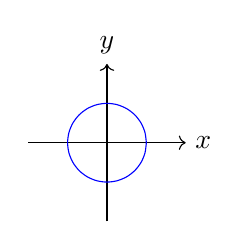
\begin{tikzpicture}
              \draw[->] (-1, 0) -- (1, 0) node[right] {$x$};
              \draw[->] (0, -1) -- (0, 1) node[above] {$y$};
              \draw[scale=0.5, domain=0:pi, smooth, variable=\t, blue]  plot ({cos(2*\t*180/pi)},{sin(2*\t*180/pi)});
            \end{tikzpicture}
          \end{center}
          Using the same technique as (a) to determine the direction of motion with the above table we see that the motion begins in quadrant 1, goes up
          to quadrant 2, down to quadrant 3, and up to quadrant 4.
    \item $x^2-1=t=y^2$ so,
          \begin{center}
            \begin{tikzpicture}
              \draw[->] (-2, 0) -- (2, 0) node[right] {$x$};
              \draw[->] (0, -0.5) -- (0, 2) node[above] {$y$};
              \draw[scale=0.5, domain=1:3, smooth, variable=\x, blue, *->]  plot ({\x}, {sqrt(\x*\x-1)});
              \draw[scale=0.5, domain=-3:-1, smooth, variable=\x, blue, <-*]  plot ({\x}, {sqrt(\x*\x-1)});
            \end{tikzpicture}
          \end{center}
          Here again using the table method we see that the motion follows the graph from left to right, becoming undefined outside of our range for $t$ which is
          not an issue as it is not motion that we would care about even if it existed, then continuing to follow the graph from left to right.
          \begin{displaymath}
            \begin{array}{|c|c|c|}
              t & x           & y \\
              \hline
              0 & \pm1        & 0 \\
              1 & \pm\sqrt{2} & 1 \\
              2 & \pm\sqrt{3} & 2 \\
            \end{array}
          \end{displaymath}
  \end{enumerate}
\end{soln}

% PROBLEM 2
\begin{problem} Find a parametrization for the line segment with endpoints $(-1, -3)$ and $(4, 1)$
\end{problem}
\begin{soln}
We can use the fact that the parametric equation of a line passing through two points is given by its direction vector times $t$ plus a point on the line. The direction vector
is $(4,1)-(-1,-3)=(5,4)$ and either of the given points lie on the line so the parametrization is $(4,1)+(5,4)t\implies x=5t+4,\, y=4t+1$
\end{soln}

% PROBLEM 3
\begin{problem} Find an equation for the line tangent to the curve at the point defined by the given value of $t$. Also, find the value of $\displaystyle\frac{d^2y}{dx^2}$ at this point.
  \begin{enumerate}[label=(\alph*)]
    \item $x=2\cos(t)$, \qquad $y=2\sin(t)$, \qquad $t=\frac{\pi}{4}$
    \item $x=\frac{1}{t}$, \qquad $y=\ln(t)-2$, \qquad $t=1$
  \end{enumerate}
\end{problem}
\begin{soln}~
  \begin{enumerate}[label=(\alph*)]
    \item $(x,y)=\left(\sqrt{2},\sqrt{2}\right)$, $\left(x^\prime,y^\prime\right)=\left(-\sqrt{2}, \sqrt{2}\right)$ so the line is $\left(\sqrt{2},\sqrt{2}\right)+\left(-\sqrt{2}, \sqrt{2}\right)t$.
    $\displaystyle\frac{d^2y}{dx^2}=\frac{d\left(\frac{dy}{dx}\right)}{dx}=\frac{\frac{d\left(\frac{dy}{dx}\right)}{dt}}{\frac{dx}{dt}}=
    \frac{\frac{d}{dt}\left[\cot(t)\right]}{2\sin(t)}=\frac{-\csc^2(t)}{2\sin(t)}=\eval{-\frac{1}{2\sin^3(t)}}_{\frac{\pi}{4}}=-\sqrt{2}$
    \item $(x,y)=(1,-2)$, $(x^\prime,y^\prime)=(-1, 1)$, so the line is $(1,-2)+(-1, 1)t$. $\displaystyle\frac{dy}{dt}=\frac{1}{t},\,\frac{dx}{dt}=-\frac{1}{t^2}\implies \frac{dy}{dx}=-t\implies 
    \frac{d^2y}{dx^2}=\frac{\frac{d}{dt}\left[-t\right]}{-\frac{1}{t^2}}=\eval{t^2}_{1}=1$
  \end{enumerate}
\end{soln}
\end{document}